\documentclass[12pt]{article}
%Gummi|065|=)
\usepackage{amsmath, amsfonts, amssymb}
\usepackage[margin=0.5in]{geometry}
\usepackage{xcolor}
\usepackage{graphicx}

\newcommand{\off}[1]{}
\DeclareMathSizes{20}{30}{20}{18}

\newcommand{\two }{\sqrt[3]{2}}
\newcommand{\four}{\sqrt[3]{4}}


\usepackage{tikz}

\title{What is Quiver W-Algebra?}
\author{John D Mangual}
\date{}
\begin{document}

\fontfamily{qag}\selectfont \fontsize{12.5}{15}\selectfont

\maketitle

\noindent Here is another situation where I must play ``follow the leader".  Between Pestun, and Kimura, and Nekrasov there's a discussion fo the $qq$-characters and these W-algebras.\footnote{An ``algebra" is just anything with a reasonable addition and multiplication. There are lots and lots of algebras we can use and study. It could be anything.  Yet, I'm confident Vasily knows what he's doing.  Why these?  and more importantly, how can I link these to the stuff that I care about? or to the big discussion?} \\ \\
Why does Pestun and Kimura extend W-algebra in this way?  The only sentence that resonates with me in any way from the intro is ``{\color{red!50!orange}our construction is orthogonal to AGT construction}".  What is AGT?  It is the definition of a conformal field theory, but it is also the literature -- all the research papers that are called ``AGT".  Tody, our discussion will be orthogonal to that. \\ \\
Literally a quiver is a collection of arrows. \\ \\ 
A \textbf{quiver} $\Gamma$ is a set of nodes $\Gamma_0$ and edges $\Gamma_1$.  An \textbf{edge}  from $i$ to $j$ is denoted: $e: i \to j$. \\ \\
A quiver defins a matrix of size $|\Gamma_0 \times \Gamma_0|$ with entries, counting the left and right arrows:
$$ c_{ij} = 2 \delta_{ij} - \# (e: i \to j) - \# (e: j \to i) $$
called the \textbf{quiver Cartan matrix}. 
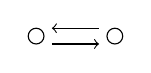
\begin{tikzpicture}
\draw (0,0) circle (0.1);
\draw (1,0) circle (0.1);
\draw[->] (0+0.2,-0.1)--(1-0.2,-0.1);
\draw[<-] (0+0.2,+0.1)--(1-0.2,+0.1);
\end{tikzpicture}
.  Next some quiver jargon:
\begin{itemize}
\item If $c_{ij} = c_{ji}$ ($\# \text{left-pointing arrows}=\# \text{right-pointing arrows}$) the quiver is ``simply laced"
\item If $c_{ij} \neq c_{ji}$ ever, the quiver is ``non-simply laced". 
\end{itemize}
The simply-laced case seems to be old news.  It's not.  We'll discuss both. \\ \\
If the quiver does not have any loops, all diagonal elements $c_{ii} = 2$ (since $\# (i \to i) = 0$).  The Kac-Moody algebras $\mathfrak{g}(\Gamma)$ are ubiquitous in physics.\footnote{``Ubiquitous" is ubiquitous in physics.  In Spanish, the word \textit{ubicar} just means ``located", instead of ``everywhere".} 
\fontfamily{qag}\selectfont \fontsize{10}{15}\selectfont
\begin{quotation}
In mathematics, a \textbf{Kac-Moody algebra} (named for {\color{green!50!white!80!black}Victor Kac} and {\color{blue!50!white}Robert Moody}, who independently discovered them) is a Lie algebra, usually infinite-dimensional, that can be defined by generators and relations through a generalized Cartan matrix. These algebras form a generalization of finite-dimensional semisimple Lie algebras, and many properties related to the structure of a Lie algebra such as its root system, irreducible representations, and connection to flag manifolds have natural analogues in the Kac-Moody setting. \\ \\
A class of Kac-Moody algebras called affine Lie algebras is of particular importance in mathematics and theoretical physics, especially conformal field theory and the theory of exactly solvable models. Kac discovered an elegant proof of certain combinatorial identities, the Macdonald identities, which is based on the representation theory of affine Kac-Moody algebras. \hfill (Wikipedia)
\end{quotation}
\fontfamily{qag}\selectfont \fontsize{12.5}{15}\selectfont
These constructions are rather bland.  We need them to define the \textbf{fractional quiver}.
\newpage

%\noindent I can't stand it !! Make it stop !! Oh God, please make it stop !! \\ \\
\noindent After that unbearable math intro, the physics definition offers us a lot more context.  Just, anything to hold on to.  The examples in Section \textbf{4} look completely tangible and rather fun: \\ \\
\textbf{\#1} $BC_2$ quiver
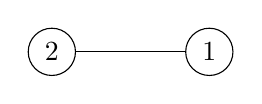
\begin{tikzpicture}
\draw (0,0) circle (0.3);
\node at (0,0) {2};
\draw (2,0) circle (0.3);
\node at (2,0) {1};
\draw (0+0.3,0)--(2-0.3,0);
\end{tikzpicture} has a ``mass-deformed" Cartan matrix:
$$ \left(  \begin{array}{ll} 
1 + \;\; q_1^{-1}q_2^{-2} & - \mu^{-1} \\ 
\hspace{0.1in}-\mu \; q_1^{-1}q_2^{-1}(1+q_2^{-1}) & \;\;\;1 + q_1^{-1}q_2^{-1}
\end{array} \right) \longrightarrow 
\left(  \begin{array}{rr} 
2 & -1 \\ -2 & 2
\end{array} \right)
$$
\textbf{\#2} 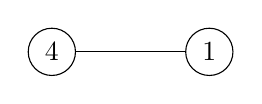
\begin{tikzpicture}
\draw (0,0) circle (0.3);
\node at (0,0) {4};
\draw (2,0) circle (0.3);
\node at (2,0) {1};
\draw (0+0.3,0)--(2-0.3,0);
\end{tikzpicture} the authors call ``affine fractional quiver" with a little more algbra:
$$ \left(  \begin{array}{ll} 
1 + \;\; q_1^{-1}q_2^{-4} & - \mu^{-1} \\ 
\hspace{0.1in}-\mu \; q_1^{-1}q_2^{-1}(1+q_2^{-1}+q_2^{-2} + q_2^{-3}) & \;\;\;1 + q_1^{-1}q_2^{-1}
\end{array} \right) \longrightarrow 
\left(  \begin{array}{rr} 
2 & -1 \\ -4 & 2
\end{array} \right)
$$
\textbf{\#3} 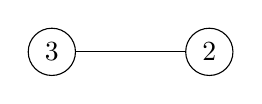
\begin{tikzpicture}
\draw (0,0) circle (0.3);
\node at (0,0) {3};
\draw (2,0) circle (0.3);
\node at (2,0) {2};
\draw (0+0.3,0)--(2-0.3,0);
\end{tikzpicture} the authors call ``hyperbolic fractional quiver"
$$ \left(  \begin{array}{ll} 
1 + \;\; q_1^{-1}q_2^{-3} & - \mu^{-1} \\ 
\hspace{0.1in}-\mu \; q_1^{-1}q_2^{-1}(1+q_2^{-1}+q_2^{-2} ) & \;\;\;1 + q_1^{-1}q_2^{-1}
\end{array} \right) \longrightarrow 
\left(  \begin{array}{rr} 
2 & -2 \\ -3 & 2
\end{array} \right)
$$
This helps us understand what Cartan matrices were all about.  There are $|\Gamma_0| = 2$ notes in each case, and the Cartan matrix is $2 \times 2$.  \\ \\
The $d$-fractional gauge theory on $\mathbb{C}^2$ involves a ring $R = \mathbb{C}[z_1, z_2] $.  At each node, the ring gets replaced by $R_ i= \mathbb{C}[z_1, z_2^{d_i}]$.  Equivariant gauge theory counts $R_i$ ideals.\footnote{Let $R$ be a ring (such as $\mathbb{C}[z_1, z_2]$.  An \textbf{ideal} is a set $\mathfrak{a} \in R$ such that
\begin{itemize}
\item $0 \in \mathfrak{a}$
\item $a,b \in \mathfrak{a}$ implies $a+b \in \mathfrak{a}$
\item $x \in R$ and $a \in \mathfrak{a}$ implies $xa \in \mathfrak{a}$.
\end{itemize} 
This is taken from a Commutative Algebra textbook (e.g. \texttt{http://web.mit.edu/18.705/www/12Nts-2up.pdf})} \\ \\
Once there is a ring you are intersted in, we can consult a Commutative Algebra or Scheme Theory textbook.  Algebraic Geometry really was supposed to be, just Algebra + Geometry
\begin{itemize}
\item we know what Algebra is
\item we know what Geometry is
\end{itemize}
it seems really plausible one might try to solve a geometry problem with algebra (and less frequently the other way around).  And, the great Algebraic Geometers understood that. This is why I really like the textbook of Hodge + Pedoe {\color{red!50!orange}Methods of Algebraic Geometry} and maybe {\color{black!50!white}The Red Book of Varieties and Schemes} by Mumford. \\ \\
I look at a ring like $\mathbb{C}[z_1, z_2]$ and think I know everything there is and could be on that subject. \\ On page 3 of Pestun-Kimura they talk about \textbf{observable sheaves} on the moduli space of instantons associatted to $R_i = \mathbb{C}[z_1, z_2^d]$ \\ \\
This is a great time to review the entire Equivariant Gauge Theory framework presented in Book 1.

\newpage

\noindent \textbf{5/16} Quiver Gauge Theories. \\ \\
Pestin, generously lets us examine all possible quivers (cuz I don't know any better).  And there will be a Cartan matrix 
$$ c_{ij} = 2 - \# (e: i \to j) - \# (e: j \to i)$$
and there is a Kac-Moody algebra $\mathfrak{g}_\Gamma$ in some way I don't know how to do. \\ \\
``Space-Time" is a complex variety\footnote{I do not know what ``complex variety" here means, if it is in Zariski topology, or more likely the topology inherited from $\mathbb{C}$.} $\mathcal{S}$ with structure sheaf $\mathcal{O}_\mathcal{S}$.   And now there is this category $\text{Coh}(\mathcal{S})$ of ``coherent sheaves" on $\mathcal{S}$. 
\begin{itemize}
\item coherent sheaf
\item category of $\mathcal{O}_\mathcal{S}$-modules
\end{itemize} 
These are \$500 objects we are looking at today, just a bit out of my reach. We ask for all coherent sheaves:
$$ \mathfrak{M}(\Gamma, \mathcal{S}) = \text{Coh}(\mathcal{S})_\Gamma / \text{Aut}\big[\text{Coh}(\mathcal{S})_\Gamma \big] $$
is the moduli space of $\Gamma$-quiver sheaves on $\mathcal{S}$. 
\begin{itemize}
\item we don't just want coherent sheaves on the variety $\mathcal{S}$ we want {\color{red!50!yellow}quiver gauge theories} $\text{Rep}\big(\Gamma, \text{Coh}(\mathcal{S})\big)$ 
\begin{itemize}
\item Each node $i$ is sent to a sheaf $\mathcal{Y}_i$ on $\mathcal{S}$
\item Each arrow $e: i \to j$ is sent to an element of $\text{Hom}_{\mathcal{O}_\mathcal{S}}(\mathcal{Y}_i, \mathcal{Y}_i)$.
\end{itemize}
\item ``Hom" is always kind of ambiguous.  In $\textbf{Vect}$ (vector spaces) it's a matrix, in $\textbf{Group}$ it counts homomorphisms, on $\textbf{Set}$ it counts bijections.  And there is Hom for many other situations.
\item Pestun is the expert on $\mathcal{N}=2$ gauge theory.  So just a few hints:
\begin{itemize}
\item Each node $i$ is sent to a {\color{red!50!green}gauge connection} $\mathcal{Y}_i$ in the {\color{red!30!green}vector multiplet}  on $\mathcal{S}$
\item Each arrow $e: i \to j$ is sent to {\color{red!70!green}bifundamental field} $\text{Hom}_{\mathcal{O}_\mathcal{S}}(\mathcal{Y}_i, \mathcal{Y}_i)$.
\end{itemize}
\end{itemize}
In Physics, complicated stuff is happening in the world.  Sheaves, derived categories \dots \\ These \$1000 objects offer us language to describe it.  \\ \\
Before I go here is the virtual tangent bundle of the tangent stack:
$$ T_\mathcal{Y}\mathfrak{M}(\Gamma, \mathcal{S})^\bullet = \bigoplus_{(e:i\to j)\in \Gamma_1} \text{Ext}_{\mathcal{O}_\mathcal{S}}^\bullet (\mathcal{Y}_i, \mathcal{Y}_i) \oplus \bigoplus_{i \in \Gamma_0} \text{Ext}_{\mathcal{O}_\mathcal{S}}^{\bullet + 1}(\mathcal{Y}_i, \mathcal{Y}_i) $$
% This version of Supersymmetric Gauge Theory has suppressed the supersymmetry and localization computations. 

\newpage

\noindent \textbf{5/18} This article is surpisingly dense for such a short discussion.  Good effective writing is like that, covers a lot of ground very succinctly. \\ \\
The formula is that partition function is the Euler characteristic of moduli space of sheaves.  
$$ Z_\text{T}(\Gamma, \mathcal{S}) = \sum_{n \in \mathbb{Z}} (-1)^n \mathrm{ch}_\text{T} H^n \big( \mathfrak{M}(\Gamma, \mathcal{S})_\gamma , \mathcal{O}_{\mathfrak{M}(\Gamma, \mathcal{S})_\gamma} \big) $$
I have on idea what these things are.
\begin{itemize}
\item fundamental matter (skip)
\item local observables (skip)
\item extended partition function (skip)
\item localization (skip)
\item partition funtion (hundreds of definitions)
\item holomorphic equivariant Euler characteristic 
\item topological sector $\gamma$ (of the quiver moduli space) a.k.a. the ``charge"
\end{itemize}
I didn't say what a Chern character or a structure sheaf were.  
What remains of this paper is a little bit odd.  We only evaluate a few ``spacetimes".  \begin{itemize}
\item $\mathcal{S} = \mathbb{C}^2$ 
\item $\mathcal{S} = \mathbb{C}_{q_1,\,q_2}$ (a doubly twisted copy of $\mathbb{C}$)
\end{itemize}
For me, these correspondences are somewhat lacking in concreteness.  \\ \\
Here is one correspondence the equiver is 
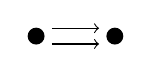
\begin{tikzpicture}
\draw[fill=black] (0,0) circle (0.1);
\draw[fill=black] (1,0) circle (0.1);
\draw[->] (0+0.2,0.1)--(1-0.2,0.1);
\draw[->] (0+0.2,-0.1)--(1-0.2,-0.1);
\end{tikzpicture} and matrix $\left[\begin{array}{rr} 2 & -2 \\ -2 & 2 \end{array}\right]$ and $\mathfrak{g}_\Gamma$ is an affine Lie algebra.  This is the $\mathrm{sinh}$-Gordon theory on the disc $\mathbb{C}^\times \backslash \{ 0\}$. The examples where somewhat spare and \dots don't do this to me. \\ \\
There is a lot of discussion on $\mathbb{C}^2$ that is what he wanted to focus on.  This is flat 4-dimensional space-time.  This is the world we live in: length, width, height, time.  \\ \\
Looks like $\mathbb{C}^2$ is all we can get. There is a lot. We can shift between the architecture and the computations.  Judging from the bibliography, it may have taken Pestun + Kimura some time to figure out for themselves what to do with a situation. \\\\
I am myself not in a position to judge until I try it for myself.

\newpage

\noindent \textbf{5/20} Let $\mathbf{Q}$ be the fiber to the cotangent bundle of $\mathcal{S} = \mathbb{C}^2$ at $o \in \mathbb{C}^2$. They could just say these are just two complex numbers.  The cotangent space of $\mathbb{C}^2$ is itself:
$$  \mathbf{Q} = T_0^\vee \mathcal{S} \simeq \mathbb{C}^2 $$
Abstract algebraic like that, we're saying that a cotangent vector is specified by two numbers.  Cotangent space probabily just means we have to specifiy a position and momentum
$$ \mathbf{x} \in \mathbb{C} \text{ and }  \mathbf{p} \in \mathbb{C}  \text{ so that }(\mathbf{x},\mathbf{p}) \in \mathbb{C}^2 $$
I would have thought position and momentum would combine as two vector.  After all $\mathbf{p} = m \mathbf{v}$ where $\mathbf{v} = \frac{d\mathbf{x}}{dt}$. \\ \\
In Lagrange formalism $L = T - V  = \text{kinetic} - \text{potential}$.  After you do enough mechanics problems (we're faking that we have\dots) who knows what the positions and momentums were, but we can describe a physics system in terms of various paramters:
$$ L = L(q) \text{ with } \dot{q} = \frac{\partial L}{\partial q}$$
and when you solve it the right way, you can get something like $\mathbf{F} = m \mathbf{a}$.  Now, momentum behaves like a co-vector:
$$ q \mapsto f(q) \text{ then }\dot{q} \mapsto \frac{\partial L}{\partial f(q)}
= \frac{\partial L}{\partial q} \frac{\partial q}{\partial f}
= \frac{\partial L}{\partial q} \Big(\frac{\partial f}{\partial q}\Big)^{-1} $$
whoops!  Now the derivative is upside-down! So here $(\,\cdot\,)^{-1}$ means reciprocal not inverse, but if it's any consolation:
$$ \frac{df^{-1}}{dq} = \frac{1}{\frac{df}{dq}} = \Big( \frac{df}{dq} \Big)^{-1} $$
and in this way, Lagrangian mechanics looks a tiny bit like category theory.  \\ \\
Unfortunately, Lagrange and his students stopped using geometry in his mechanics problems.  And what a can of worms that opened up! \\ \\
Hamilton of course had $H = L + V$ and the situation is almost the same. \\  Let's continue nice and slow.

\vfill

\begin{thebibliography}{}

\item Taro Kimura, Vasily Pestun \textbf{Fractional Quiver W-algebras} \texttt{arXiv:1705.04410}

\item Taro Kimura, Vasily Pestun \textbf{Quiver Elliptic W-algebras} \texttt{arXiv:1608.04651}

\item Taro Kimura, Vasily Pestun \textbf{Quiver W-algebras} \texttt{arXiv:1512.08533}

%\item Nikita Nekrasov. \textbf{BPS/CFT correspondence: non-perturbative Dyson-Schwinger equations and qq-characters.} \texttt{arXiv:1512.05388}





\end{thebibliography}

\end{document}